\section{Optimierung der Parameter}
\label{Parameteroptimierung}
Um die Ergebnisse der Klassifikation zu verbessern, wurden die Parameter für den J48 Algorithmus optimiert. Dabei handelt es sich um die Parameter C und M, deren Einfluss in Kapitel \ref{Klassifikation} beschrieben wurde. Der Suchraum wurde diskretisiert und anschließend wurden 1000 Kombinationen der Parameter getestet. Dabei wurden in die Featurevektoren alle beschriebenen Features eingetragen. Getestet wurde mit 5000 Sudokus aus fünf verschiedenen Klassen mit 10-Fold cross validation. Als Maß für die Güte der Klassifikation wurde der prozentuale Anteil der korrekt klassifizierten Sudokus verwendet.\\

\begin{figure}[H]
    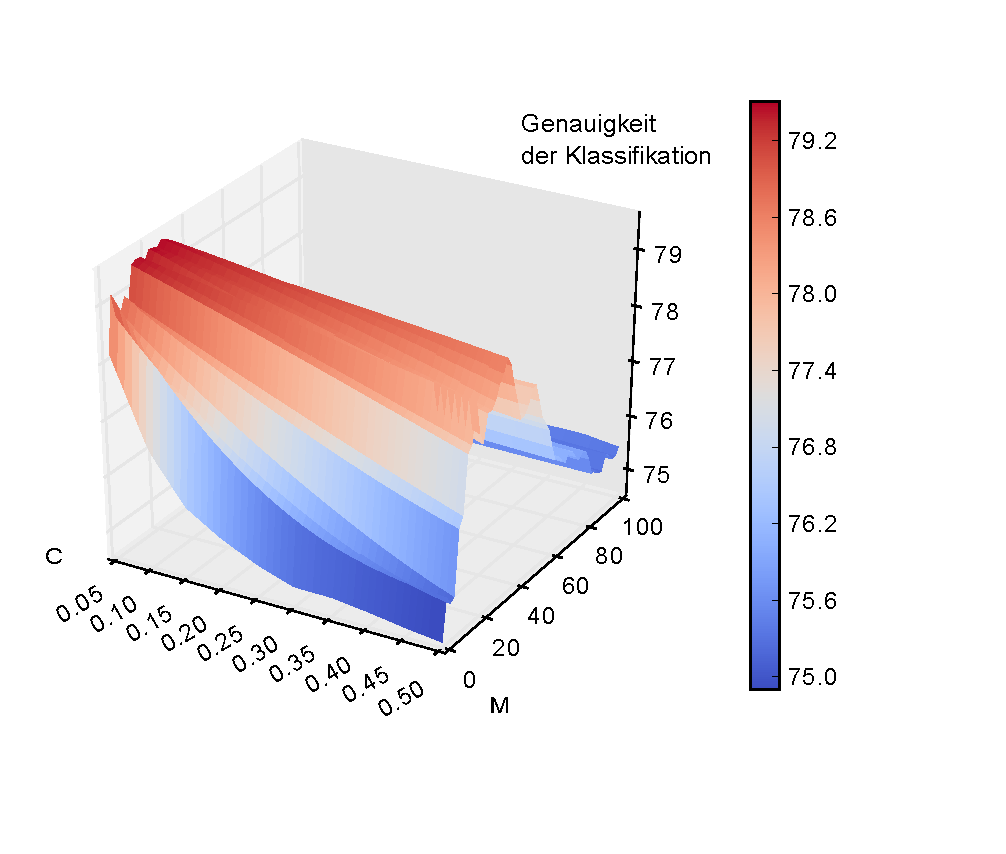
\includegraphics[scale=0.9]{./img/parameter.eps}
    \caption{Anzahl der korrekt klassifizierten Sudokus mit verschiedenen Kombinationen von C und M}
\end{figure}

\noindent Wie die in \textbf{Abbildung 5.1} abgebildeten Ergebnisse zeigen, liegen die optimalen Parameter für den Algorithmus für C bei 0.1 und für M bei 30. Dies gilt nur für die in diesem Test verwendeten Sudokus und Featurevektoreinträge, für neue Sudokus können die optimalen Parameter variieren.